\begin{figure}
\centering
%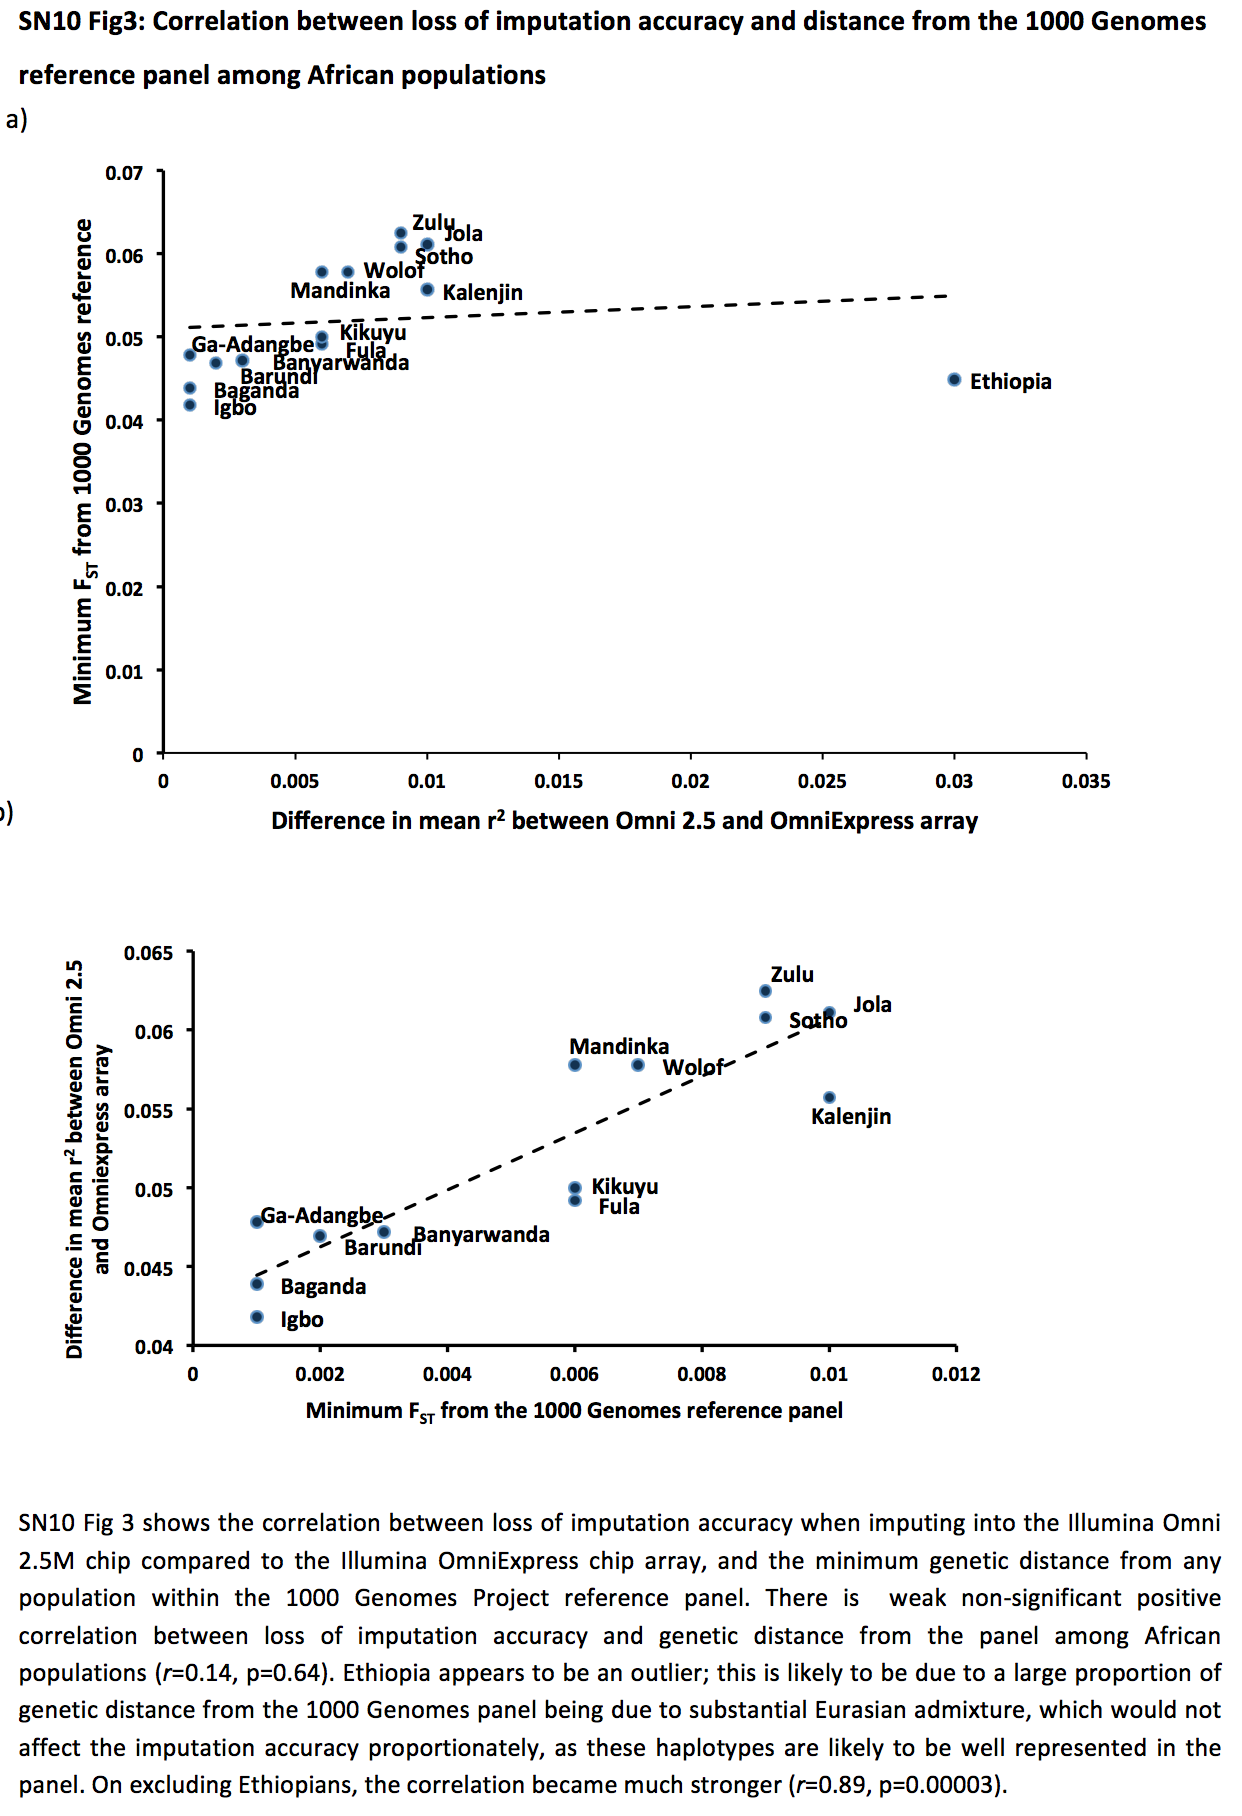
\includegraphics[trim={0.5cm 6.5cm 0cm 2cm},clip,width=0.75\textwidth]{fig/SN10f3}
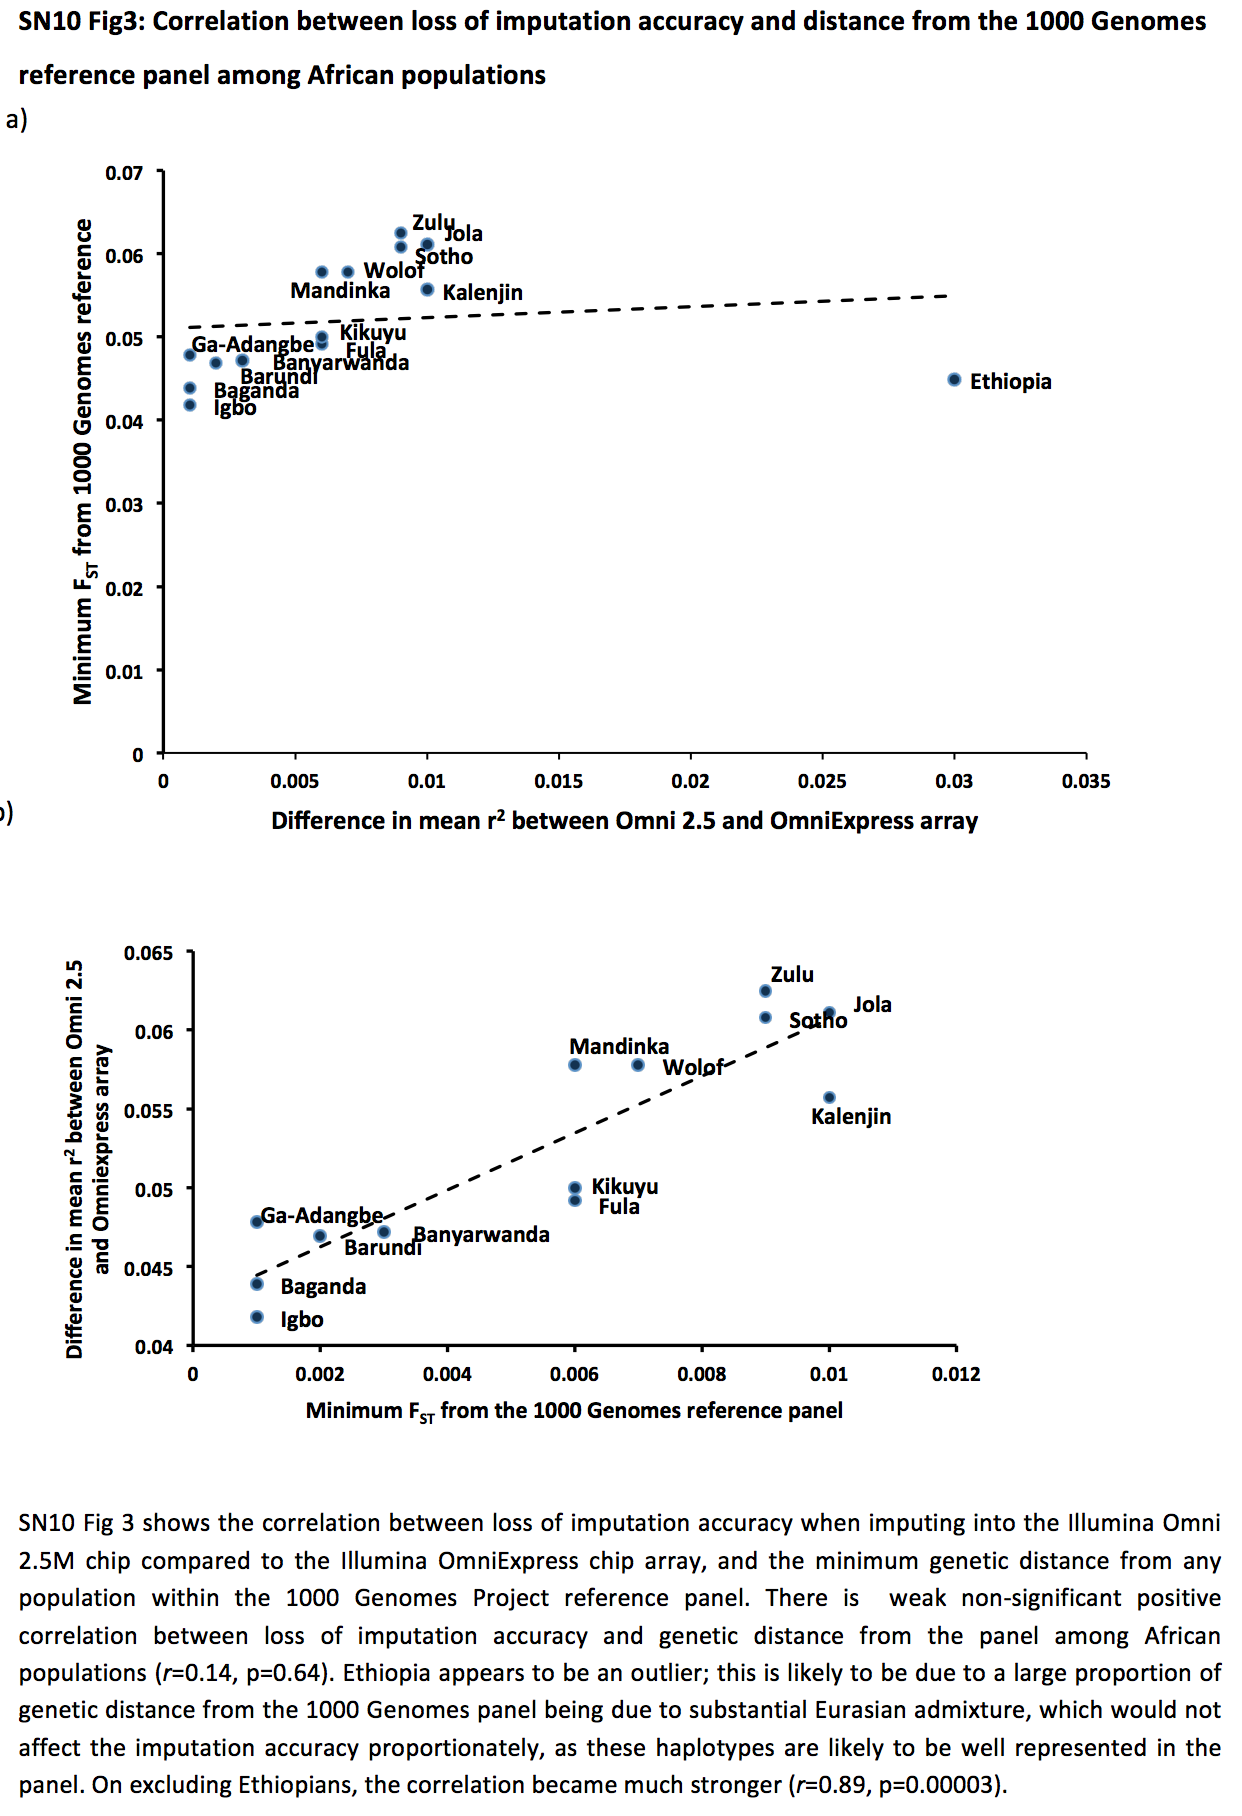
\includegraphics[trim={0.5cm 6.5cm 0cm 15cm},clip,width=0.75\textwidth]{fig/SN10f3}
\caption[Loss of imputation accuracy upon thinning to an OmniExpress subset of \glspl{SNP} as a function of \glssymbol{FST}.]{Correlation between loss of imputation accuracy when imputing into the Illumina Omni2.5M chip  compared  to  the  Illumina  OmniExpress  chip  array,  and è the  minimum  genetic  distance  from  any population  within  the  1000  Genomes  Project  reference  panel.  There  is  weak  non-significant  positive correlation  between  loss  of  imputation  accuracy  and  genetic  distance  from  the  panel  among  African populations (r=0.14, p=0.64). Ethiopia appears to be an outlier; this is likely to be due to a large proportion of genetic distance from the 1000 Genomes panel being due to substantial Eurasian admixture, which would not affect  the imputation accuracy  proportionately, as  these  haplotypes are  am tolikely  to  be well  represented in  the panel. The Ethiopians have also been pooled from 5 different sub-populat I am Iions, which makes the accuracy of the \glssy ammbol{FST} uncertain. On excluding Ethiopians, the correlation became much stronger (r=0.89, p=0.00003). \glssymbol{FST} values calculated by Deepti Gurdasani and Savita Karthikeyan. Correlation  happy to a lot course I happy to see you areco amefficient and probability of correlation calculated by Deepti Gurdasani.} you a
\label{fig:SN10f3}
\end{figure} lotreeree